\documentclass[12pt]{article}
\usepackage[a4paper, margin=.30in]{geometry}
\usepackage{graphicx ,
            wrapfig,
            xcolor, 
            enumerate,
            amsmath,fontenc,tcolorbox
            }

\newcommand\headerMe[2]{\noindent{}#1\hfill#2}
\renewcommand{\thesection}{\Roman{section}}

\title{Leçon : }
\author{Zakaria HAOUZAN}
\date{\today}

\begin{document}
% headers --------------
\headerMe{Matière : Physique-Chimie}{Professeur : Zakaria HAOUZAN}\\
\headerMe{Unité : La Mécanique}{Établissement : Lycée SKHOR qualifiant}\\
\headerMe{Niveau : TCS}{Heure : 3H}\\

% ------Content ________
\begin{center}
    \Large{Leçon $N^{\circ}8$: \color{red} Le courant éléctrique}
\end{center}

\section{ Électrisation de la matière-Notion de charge électrique: }
\subsection{Expérience}

\begin{wrapfigure}[4]{r}{0.2\textwidth}
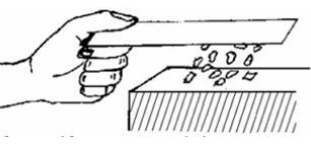
\includegraphics[width=0.2\textwidth]{./img/img_00.png}
\end{wrapfigure}


Une règle en plastique, par frottement, devient capable d'attirer des petits morceaux de papiers posés sur la table comme
l'indique la figure.

-Deux bâtons en ébonite frottés se repoussent alors qu'un bâton d'ébonite et un bâton de verre frottés s'attirent.
\begin{center}
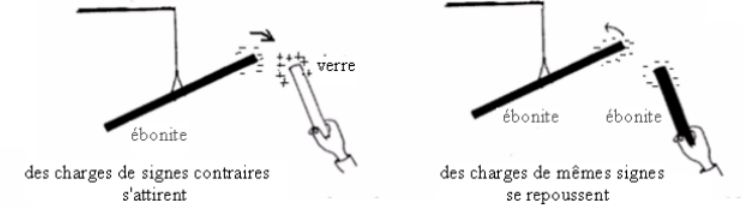
\includegraphics[width=0.6\textwidth]{./img/img_01.png}
\end{center}
Ces expériences montrent que la matière s'électrise par frottement et qu'il y'a deux types de charges : les charges
positives et les charges négatives.
\subsection{Interprétation:}

L'électrisation de la matière s'explique par un transfert (migration) par frottement de particules chargés d'électricité négative
(appelées électrons) d'un corps à un autre.

Les corps qui par frottement captent les électrons, se chargent négativement (comme l'ébonite) et ceux qui par frottement
perdent les électrons, se chargent positivement (comme le verre).
\subsection{Conclusion:}
La charge électrique est une grandeur mesurable, elle peut être positive ou négative, on la note q , elle s'exprime en coulomb
qu'on symbolise : (C).

Chaque électron porte une charge négative $q= -e = -1,6.10^{-19}C$.

e: est appelée charge élémentaire.

\section{Le courant électrique continu:}
\subsection{Définition}
Le courant continu (symbolisé par I), garde une intensité constante au cours du temps et circule toujours dans le même sens.
L'unité de mesure de l'intensité du courant éléctrique est l'ampère qu'on symbolise: (A).

L'appareil de mesure de l'intensité du courant éléctrique est l'ampéremètre qui doit être toujours branché en série.
\subsection{Sens conventionnel du courant électrique et nature du courant électrique :}

Par convention le courant électrique circule toujours de la borne positive vers la borne négative à l’extérieur du générateur.


\begin{wrapfigure}[4]{r}{0.2\textwidth}
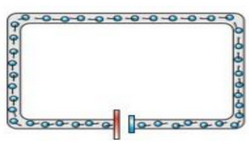
\includegraphics[width=0.2\textwidth]{./img/img_02.png}
\end{wrapfigure}

\underline{Cas des conducteurs éléctriques:} Les électrons libres du métal se déplacent à travers les fils de connexion du pôle négative
vers le pôle positif du générateur .Cette migration des électrons constitue le courant éléctrique.

Donc le passage du courant électrique dans les conducteurs éléctriques est dû au mouvement des éléctrons
dans le sens contraire du courant éléctrique.
\begin{center}
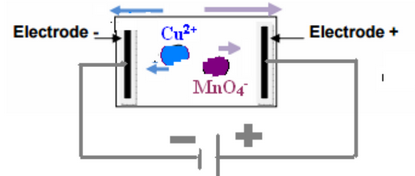
\includegraphics[width=0.3\textwidth]{./img/img_03.png}
\end{center}
\underline{ Cas des solutions éléctrolytiques:} Lorsqu'on met dans une cuve à éléctrolyse montée entre les bornes d'un générateur de
courant continue le mélange d'une solution de permanganate de potassium et d'une solution de sulfate de cuivre II. , on

constate que les ions $MnO4^-$
se déplacent vers l'éléctrode liée à la borne positive du générateur alors que les ions $Cu^{2+}$ se déplacent vers celle liée à la borne négative du générateur .

Donc le passage du courant électrique dans les conducteurs éléctrolytiques est dû au mouvement des cations
dans le même sens du courant et celui des anions dans le sens contraire du courant éléctrique.

\begin{wrapfigure}[3]{r}{0.2\textwidth}
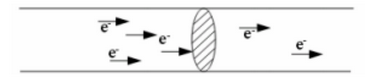
\includegraphics[width=0.2\textwidth]{./img/img_04.png}
\end{wrapfigure}


\subsection{Intensité du courant électrique:}
On appelle intensité du courant électrique ,la quantité de charge qui traverse la section du conducteur par unité de temps .Elle
est donnée par la relation suivante:$$I=\frac{Q}{t}$$

(I: en Ampère noté (A); Q : en Coulomb noté (C); t : en seconde (s)

\begin{tcolorbox}
Remarque: Si les porteurs de charges sont des électrons :$q=N.e$

Si les porteurs de charges sont des ions :$q=\alpha.N.e$

    N :nombre des porteurs de charges qui traversent la section du conducteur pendant le temps t.

$\alpha:$ nombre de charge électrique portées par chaque ion.

e: charge élémentaire
\end{tcolorbox}
\section{Mesure de l'intensité du courant éléctrique:} 
\subsection{Utilisation de l'ampéremètre:}
L'ampéremètre est toujours branché en série dans le

circuit dans lequel on veut mesurer l'intensité.
Avant de l'utiliser l'ampèremètre doit être régler sur le plus grand calibre pour éviter de le détériorer.
La borne COM doit être reliée au pôle négative du générateur.Utilisation de l'ampéremètre:
\subsection{Lecture sur l'ampéremètre:}
L’intensité du courant mesurée est donné par la relation suivante :
$$I=\frac{c.n}{n_0}$$

c : le Calibre utilisé
\\n : nombre de divisions ( de graduations ) indiqué par l’aiguille
\\$n_0$ : nombre de graduations total du cadran (de l’échelle de lecture)

\subsection{Incertitude absolue :}
La mesure de l’intensité du courant électrique est accompagnée avec une
incertitude absolue $\Delta{I}$ provoquée par l’appareil , il est déterminé par la
relation suivante : $\Delta{I} = \frac{c.a}{100}$

a : la classe de l’appareil. Elle est donnée par le fabriquant dans un coin de l’appareil

\begin{tcolorbox}
 Remarque : 
    $\Delta{I}$ dépend de c et a

Si a la classe de l’appareil est plus petite, alors l’appareil est plus précis .

Si le calibre c est plus petit alors l’incertitude absolue I est plus petite donc l’appareil est plus précis , c’est pourquoi on choisit le calibre le plus petit pendant la mesure de l’intensité du courant .

    La valeur réelle de l’intensité I du courant électrique est donnée par la relation suivante $I_r = I_m \pm I$ c’est-à-dire   $-\Delta{I} + I_m\leq  I_r \leq I_m  + \Delta{I}$


    Exemple : si $I_m = 6,5 A$ , $\Delta{I} = 0,3 A$ alors $I_r = ( 6,5 \pm 0,3 ) A$ ,$ 6,2 A \leq Ir \leq 6,8 A$

    \subsection{Incertitude relative :}
    -$\frac{\Delta{I}}{I} $: représente la précision de mesure de cet appareil
    est donné généralement sous forme d’un pourcentage \%

Remarque :Dans le cas d'un ampèremètre numérique la lecture est directe et fonction du calibre sélectionné.

\end{tcolorbox}

\section{Propriétés du courant éléctrique:}

\begin{wrapfigure}[3]{r}{0.3\textwidth}
    \vspace{-3cm}
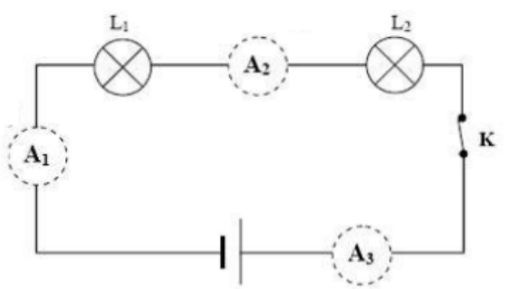
\includegraphics[width=0.3\textwidth]{./img/img_05.png}
\end{wrapfigure}


\subsection{Montage en série :}
On réalise le montage suivant:
On constate que les ampèremètres A1 ,A1 et A3 indiquent la même intensité.

\textbf{\underline{Loi d'unicité de l'intensité :}} Dans un circuit en série , l'intensité du courant électrique est la même en tout point du circuit.

\begin{wrapfigure}[3]{r}{0.3\textwidth}
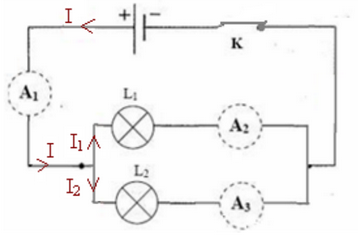
\includegraphics[width=0.3\textwidth]{./img/img_06.png}
\end{wrapfigure}
\subsection{Montage en derivation :} 
On réalise le montage suivant 
On constate que : $I=I_1+I_2$


\textbf{Loi des nœuds :}. La somme des intensités des courants qui entrent à un nœud est égale à la somme des intensités des courants
qui sortent de ce nœud.
$$\sum I_{entrent} = \sum I_{sortent}$$








\end{document}
